\chapter{Introducción}
\label{cap:capitulo1}
\setcounter{page}{1}

En este capítulo de introducción, se aborda el contexto general y específico en el que se enmarca el proyecto de diseño de un sistema de topografía mediante el uso de sensores. Se discutirá la importancia de la topografía en diferentes campos, como la construcción y la ingeniería, así como las limitaciones de los métodos tradicionales de medición topográfica. Se presentará la solución propuesta para superar estas limitaciones, utilizando diferentes herramientas e información. Además, se incluirán referencias bibliográficas que respalden la relevancia del tema y justifiquen la elección de diferentes mecanismos utilizados en el proyecto.\\

\section{Objetivo del proyecto}
\label{sec:miseccion} % etiqueta para luego referenciar esta sección

El objetivo del TFG es diseñar un sistema de topografía mediante el uso de sensores, específicamente utilizando una placa de Arduino Uno, un sensor de orientación absoluta IMU-BNO055 y un láser de alta precisión para medir distancias. Este sistema busca ofrecer una solución más precisa, rápida y eficiente en comparación con los métodos de medición topográfica tradicionales. Para lograr este objetivo, se llevará a cabo un proceso de investigación exhaustivo para seleccionar los sensores más adecuados y desarrollar un sistema integrado que pueda ser utilizado en diferentes aplicaciones. Se evaluará la precisión y eficiencia del sistema mediante pruebas y mediciones en diferentes entornos y se analizarán los resultados obtenidos para validar la efectividad del sistema de topografía propuesto.

\section{Alcance del proyecto}
\label{sec:segundaseccion}

No olvides incluir imágenes y referenciarlas, como la Figura \ref{fig:mpu-9250}.

\begin{figure} [h!]
  \begin{center}
    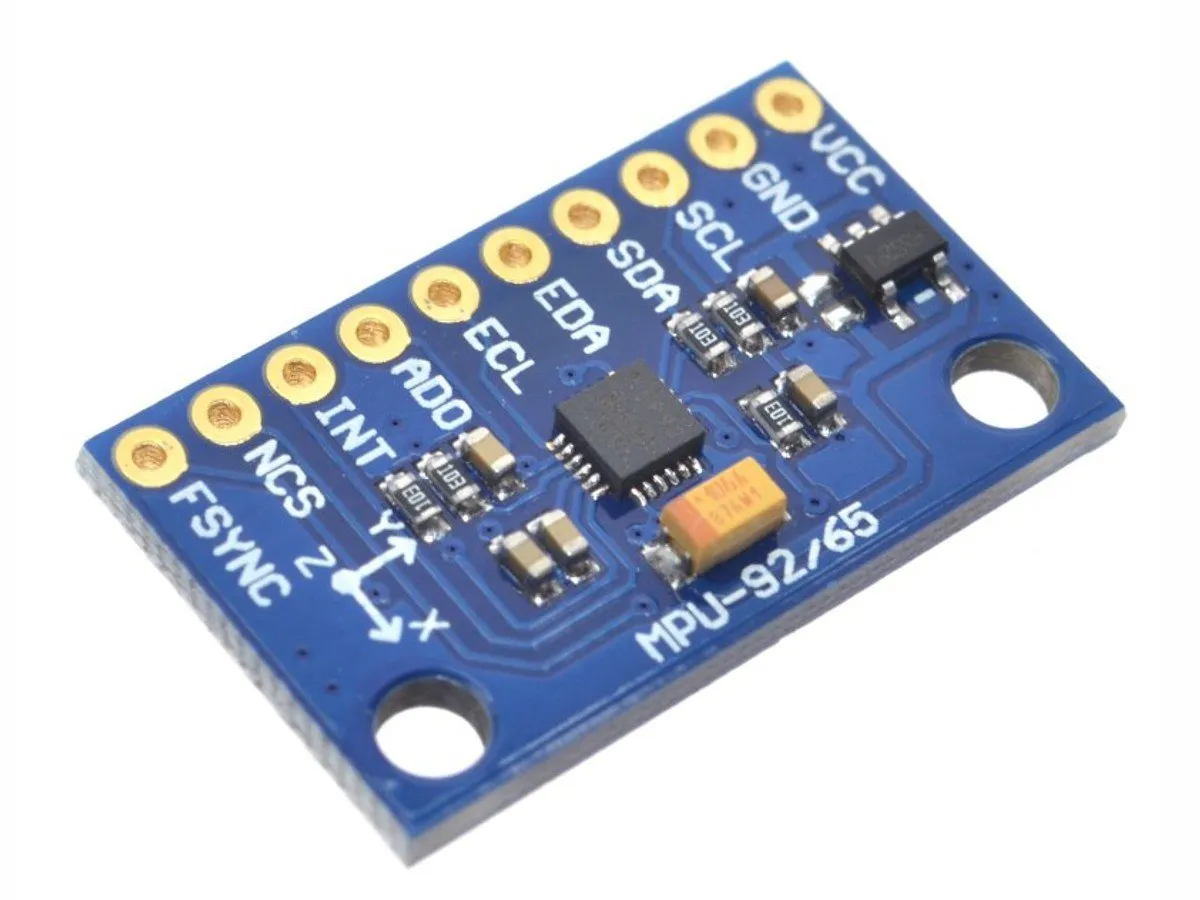
\includegraphics[width=8cm]{figs/mpu-9250}
  \end{center}
  \caption{Disposito MPU-9250.}
  \label{fig:mpu-9250}
\end{figure}\

Ni tampoco olvides de poner las URLs como notas al pie. Por ejemplo, si hablo de la Robocup\footnote{\url{http://www.robocup.org}}.

\subsection{Motivación}
\label{sec:subseccion}

En lugar de tener secciones interminables, como la Sección \ref{sec:miseccion}, divídelas en subsecciones.

Para hablar de números, mételos en el entorno \textit{math} de \LaTeX, por ejemplo, $1.5Kg$. También puedes usar el símbolo del Euro como aquí: 1.500\euro.

\subsection{Planificación}

Cuando describas una colección, usa \texttt{itemize} para ítems o \texttt{enumerate} para enumerados. Por ejemplo:

\begin{itemize}
 \item \textit{Entorno de simulación.} Hemos usado dos entornos de simulación: uno en 3D y otro en 2D.
 \item \textit{Entornos reales.} Dentro del campus, hemos realizado experimentos en Biblioteca y en el edificio de Gestión.
\end{itemize}\

\begin{enumerate}
 \item Primer elemento de la colección.
 \item Segundo elemento de la colección.
\end{enumerate}\

\paragraph{Referencias bibliográficas}
\label{sec:referencias}

Cita, sobre todo en este capítulo, referencias bibliográficas que respalden tu argumento. Para citarlas basta con poner la instrucción \verb|\cite| con el identificador de la cita. Por ejemplo: libros como \cite{vega12e}, artículos como \cite{vega19b}, URLs como \cite{vega19a}, tesis como \cite{vega18b}, congresos como \cite{vega18a}, u otros trabajos fin de grado como \cite{vega08b}.

Las referencias, con todo su contenido, están recogidas en el fichero \texttt{bibliografia.bib}. El contenido de estas referencias está en formato \texttt{BibTex}. Este formato se puede obtener en muchas ocasiones directamente, desde plataformas como \texttt{Google Scholar} u otros repositorios de recursos científicos.

Existen numerosos estilos para reflejar una referencia bibliográfica. El estilo establecido por defecto en este documento es APA, que es uno de los estilos más comunes, pero lo puedes modificar en el archivo \texttt{memoria.tex}; concretamente, cambiando el campo \verb|apalike| a otro en la instrucción \verb|\bibliographystyle{apalike}|. 




\

\

\

Y, para terminar este capítulo, resume brevemente qué vas a contar en los siguientes.
